\documentclass{beamer}

\usetheme{CambridgeUS}

\usepackage{hyperref}
\usepackage{verbatim}

\title{What Makes a Country Wealthy?}
\subtitle{Regression Analysis using World Bank Development Indicators}
\date{\today}
\subject{Statistics}

\author{K.~Chen\inst{1} \and V.~Sharma\inst{1} \and JL.~Etienne\inst{1}}

\institute[Williams College] 
{
  \inst{1}
  Statistics 202 \\
  Williams College
}

\date{\today}

% Use for TOC at subsection start:
% \AtBeginSubsection[] { \begin{frame}<beamer>{Outline} \tableofcontents[currentsection,currentsubsection] \end{frame} }


\hypersetup{
    bookmarks=true,         % show bookmarks bar?
    unicode=false,          % non-Latin characters in Acrobat’s bookmarks
    pdftoolbar=true,        % show Acrobat’s toolbar?
    pdfmenubar=true,        % show Acrobat’s menu?
    pdffitwindow=false,     % window fit to page when opened
    pdfstartview={FitH},    % fits the width of the page to the window
    pdftitle={My title},    % title
    pdfauthor={Author},     % author
    pdfsubject={Subject},   % subject of the document
    pdfcreator={Creator},   % creator of the document
    pdfproducer={Producer}, % producer of the document
    pdfkeywords={keyword1} {key2} {key3}, % list of keywords
    pdfnewwindow=true,      % links in new window
    colorlinks=true,       % false: boxed links; true: colored links
    linkcolor=red,          % color of internal links (change box color with linkbordercolor)
    citecolor=green,        % color of links to bibliography
    filecolor=magenta,      % color of file links
    urlcolor=cyan           % color of external links
}

\begin{document}

\begin{frame}
\titlepage
\end{frame}

\begin{frame}{Outline}
\tableofcontents%[pausesections]
\end{frame}


% % % % % % % % % % % % % % % % % % % %
% % % % % % % % % % % % % % % % % % % %
% % % % % % % % % % % % % % % % % % % %
\section{Research Question}

%RESPONSE
\subsection{Response of Interest}
\begin{frame}{What makes a country rich?}{Response of Interest}
  \begin{figure}
    \includegraphics[scale=0.35]{images/country_maps/map_gdp_per_capita.jpeg}
  \end{figure}
\end{frame}

\begin{frame}{Response of Interest}{Reason for ``per capita''}
\begin{itemize}
\item Two metrics for wealth:
  \begin{itemize}
  \item GDP
  \item GDP per capita
  \end{itemize}
\item Compare Japan and China (in 2012 USD)
  \begin{table}
    \begin{tabular}{| l | l | l |} \hline
      ~     & GDP (in trillions) & GDP per capita (in thousands) \\ \hline
      China & 8.2                            & 6                                         \\ \hline
      Japan & 6                              & 46                                        \\ \hline
    \end{tabular}
  \end{table}
\end{itemize}
\end{frame}

\begin{frame}{GDP per capita}{Log transform the response to move outliers}
  \begin{columns}
    \begin{column}{0.5\textwidth}
      \begin{figure}
        \includegraphics[scale=0.2]{images/histogram_plots/Response/GDP_per_capita.png}
        \caption{$Y = \textrm{GDP per capita}$.}
      \end{figure}
    \end{column}
    
    \begin{column}{0.5\textwidth}
      \begin{figure}
        \includegraphics[scale=0.2]{images/histogram_plots/Response/log_GDP_per_capita.png}
        \caption{$\ln(Y)$ removes outliers.}
      \end{figure}
    \end{column}
  \end{columns}
\end{frame}


%DATA
\subsection{Data Overview}
\begin{frame}{Downloading the Data}
  \begin{itemize}
  \item Collected from \href{http://data.worldbank.org/indicator}{The World Bank} 
  \item All countries -- Afghanistan to Zimbabwe
  \item Only two years -- 1980, 2008
    \begin{itemize}
    \item \emph{time series} problems, e.g. autocorrelation
    \end{itemize}
  \end{itemize}
\end{frame}

\begin{frame}{Long to Wide Format}
  \begin{itemize}
  \item Use the {\tt reshape} package
  \item \emph{Long} format --- what we downloaded \\
    \begin{table}
      \begin{tabular}{ | l | l | l | } \hline
	Country		& Variable		& Value \\ \hline
	Afghanistan	& GDP1980		& 2.4   \\ \hline
	Afghanistan	& GDP2008  		& 2.7   \\ \hline
	Afghanistan	& CO$_2$1980  	& 4.6   \\ \hline
	Afghanistan	& CO$_2$2008  	& 5.6   \\ \hline
      \end{tabular}
    \end{table}
    
  \item \emph{Wide} format --- what we want \\
    \begin{table}
      \begin{tabular}{| l || l | l | l | l |} \hline
	Country		& GDP1980	& GDP2008	& CO$_2$1980	& CO$_2$2008 \\ \hline
	Afghanistan	& 2.4			& 2.7			& 4.6				& 5.6 \\ \hline
        %			Albania		& 4.3			& 4.6			& 3.2				& 4.2 \\ \hline
      \end{tabular}
    \end{table}
  \end{itemize}
\end{frame}

\begin{frame}{Parcelling Data into Frames}{{\tt build.R} creates a frame per year}
  \begin{itemize}
  \item What we have: \\
    \begin{table}
      \begin{tabular}{| l || l | l | l | l |} \hline
	Country		& GDP1980	& GDP2008	& CO$_2$1980	& CO$_2$2008 \\ \hline
	Afghanistan	& 2.4			& 2.7			& 4.6				& 5.6 \\ \hline
        %			Albania		& 4.3			& 4.6			& 3.2				& 4.2 \\ \hline
      \end{tabular}
    \end{table}
    
  \item What we want (for each year): \\
    \begin{table}
      \begin{tabular}{ | l || l | l | } \hline
	Country     & GDP & CO2 \\ \hline
	Afghanistan & 2.4 & 4.6 \\ \hline
      \end{tabular}
    \end{table}
  \end{itemize}
\end{frame}

\begin{frame}{Over 1300 Indicators}
  \begin{itemize}
  \item Education
  \item Economic Policy \& Debt
  \item Finance
  \item Health
  \item Infrastructure
  \item Labor
  \item Poverty
  \item Trade
  \end{itemize}
\end{frame}



% % % % % % % % % % % % % % % % % % % %
% % % % % % % % % % % % % % % % % % % %
% % % % % % % % % % % % % % % % % % % %
% RURAL PREDICTOR
% % % % % % % % % % % % % % % % % % % %
% % % % % % % % % % % % % % % % % % % %
% % % % % % % % % % % % % % % % % % % %
\section{Rural Population Model}


\begin{frame}{{\sc Rural Population} Model}{\tt log(GDP.per.capita) $\sim$ \href{http://data.worldbank.org/indicator/SH.H2O.SAFE.RU.ZS}{rural.water} + \href{http://data.worldbank.org/indicator/SP.RUR.TOTL.ZS}{rural.population}}
  \begin{columns}
    \begin{column}{0.5\textwidth}
      \begin{itemize}
      \item wellbeing indicator
        \begin{itemize}
        \item \% of rural population w/ access to clean {\bf water}
        \end{itemize}
        \begin{figure}
	  \centering
	  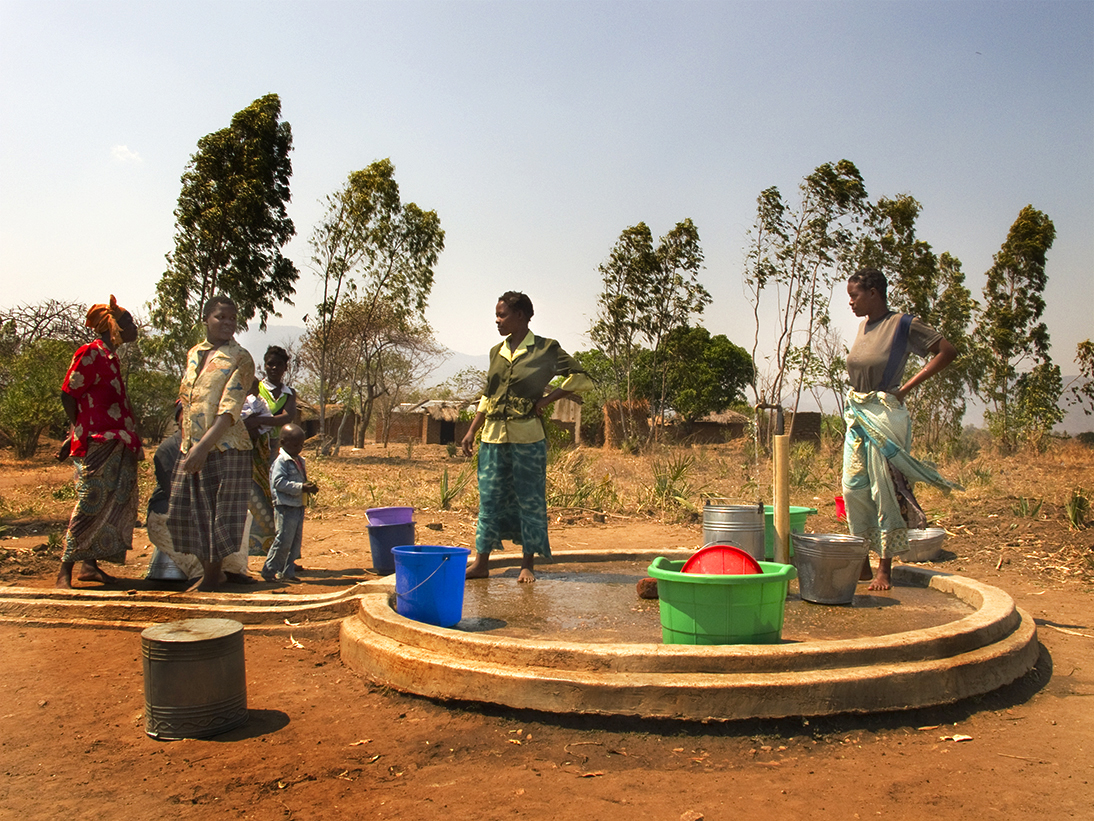
\includegraphics[scale=0.12]{images/malawi_rural_water.jpg}
	  %\caption{Rural water source in Malawi}
	\end{figure}
      \end{itemize}
    \end{column}
    
    \begin{column}{0.5\textwidth}
      \begin{itemize}
      \item production indicator
        \begin{itemize}
        \item rural {\bf population} (\% of total)
        \item countryside dwellers $\rightarrow$ farmers $\rightarrow$ produce $\rightarrow$ wealth 
        \end{itemize}
        \begin{figure}
	  \centering
	  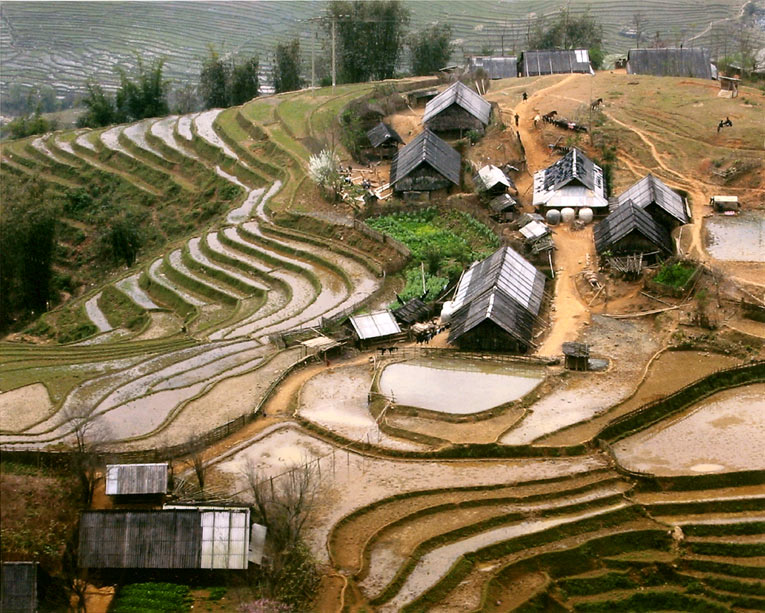
\includegraphics[scale=0.15]{images/sapa_vietnam_2003.jpg}
	  %\caption{Sapa, Vietnam 2003}
	\end{figure}
      \end{itemize}
    \end{column}
  \end{columns}
\end{frame}


\begin{frame}{{\sc Rural Population} Model}{Checking conditions (equal variance \& normality)}
    \begin{figure}
      \centering
      \includegraphics[scale=0.15]{images/condition_plots/rural.jpeg}
      \caption{Left to right: \href{http://data.worldbank.org/indicator/SH.H2O.SAFE.RU.ZS}{\tt rural.water}, \href{http://data.worldbank.org/indicator/SP.RUR.TOTL.ZS}{\tt rural.population}}
    \end{figure}
\end{frame}

\begin{frame}[fragile]{{\sc Rural Population} Regression}
\small
\begin{verbatim}
Coefficients:
                          Estimate Std. Error t value Pr(>|t|)    
(Intercept)               7.266272   0.371450   19.56   <2e-16 ***
rural.water               0.034788   0.003426   10.15   <2e-16 ***
rural.population.percent -0.036763   0.003057  -12.03   <2e-16 ***
\end{verbatim}
\begin{itemize}
\item A one-unit increase in the percentage of rural population reduces GDP per capita by 3\%.
\item $df = 175$, 36 observations deleted 
\item Adjusted R-squared:  0.7339
\end{itemize}
\end{frame}



% % % % % % % % % % % % % % % % % % % %
% % % % % % % % % % % % % % % % % % % %
% % % % % % % % % % % % % % % % % % % %
% URBAN PREDICTOR
% % % % % % % % % % % % % % % % % % % %
% % % % % % % % % % % % % % % % % % % %
% % % % % % % % % % % % % % % % % % % %
\section{Urban Population Model}

\begin{frame}{{\sc Urban Population} Model}{\tt log(GDP.per.capita) $\sim$ \href{http://data.worldbank.org/indicator/SH.H2O.SAFE.UR.ZS}{urban.water} + \href{http://data.worldbank.org/indicator/SH.STA.ACSN.UR}{urban.sanitation} + \href{http://data.worldbank.org/indicator/SP.URB.TOTL.IN.ZS}{urban.population}}
  \begin{columns}
    \begin{column}{0.5\textwidth}
      \begin{itemize}
      \item wellbeing indicators
	\begin{itemize}
	\item \% of urban population w/ access to {\bf sanitation}
	\item \% of urban population w/ access to clean {\bf water}
	  \begin{figure}
	    \centering
	    \includegraphics[scale=1.2]{images/urban_water.jpg}
	  \end{figure}
	\end{itemize}
      \end{itemize}
    \end{column}
    
    \begin{column}{0.5\textwidth}
      \begin{itemize}
      \item size indicator
        \begin{itemize}
        \item urban {\bf population} (\% of total)
        \end{itemize}
        \begin{figure}
	  \centering
	  \includegraphics[scale=0.15]{images/urban_sprawl.jpg}
	\end{figure}
      \end{itemize}
    \end{column}
  \end{columns}
\end{frame}


\begin{frame}{{\sc Urban Population} Model}{Checking conditions (equal variance \& normality)}
  \begin{itemize}
  \item {\tt urban.water} could not be improved w/ log transformation
    \begin{figure}
      \centering
      \includegraphics[scale=0.1]{images/condition_plots/urban.jpeg}
      \caption{Left to right: \href{http://data.worldbank.org/indicator/SH.H2O.SAFE.UR.ZS}{\tt urban.water}, \href{http://data.worldbank.org/indicator/SH.STA.ACSN.UR}{\tt urban.sanitation}, \href{http://data.worldbank.org/indicator/SP.URB.TOTL.IN.ZS}{\tt urban.population}}
    \end{figure}
  \end{itemize}
\end{frame}

\begin{frame}[fragile]{{\sc Urban Population} Regression}
\small
\begin{verbatim}
Coefficients:
                 Estimate Std. Error t value Pr(>|t|)    
(Intercept)      4.140821   0.198559   20.85   <2e-16 ***
urban.sanitation 0.031537   0.002881   10.95   <2e-16 ***
urban.population 0.032861   0.003058   10.75   <2e-16 ***
\end{verbatim}
\begin{itemize}
\item A one unit increase in urban population w/ access to toilets yields a 3\% increase in GDP per capita.
\item $df = 178$, 33 observations deleted 
\item Adjusted R-squared:  0.7532
\end{itemize}
\end{frame}




% % % % % % % % % % % % % % % % % % % %
% % % % % % % % % % % % % % % % % % % %
% % % % % % % % % % % % % % % % % % % %
% CLIMATE PREDICTOR
% % % % % % % % % % % % % % % % % % % %
% % % % % % % % % % % % % % % % % % % %
% % % % % % % % % % % % % % % % % % % %
\section{Climate Change Model}

\begin{frame}{{\sc Climate Change} Model}{\tt log(GDP.per.capita) $\sim$ \href{http://data.worldbank.org/indicator/EG.USE.ELEC.KH.PC}{electricity.consumption} + pollution + \href{http://data.worldbank.org/indicator/IS.ROD.PAVE.ZS}{paved.roads}}
  \begin{columns}
    \begin{column}{0.5\textwidth}
      \begin{itemize}
      \item electricity consumption (kWh per capita)
        \begin{figure}
	  \centering
	  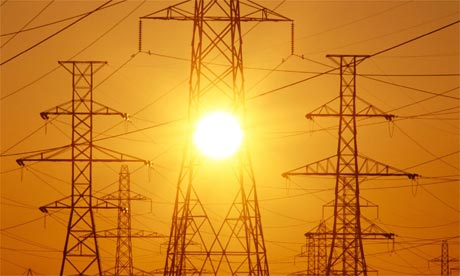
\includegraphics[scale=0.25]{images/electricity_consumption.jpg}
        \end{figure}
      \item paved roads (\% of total)
        \begin{figure}
	  \centering
	  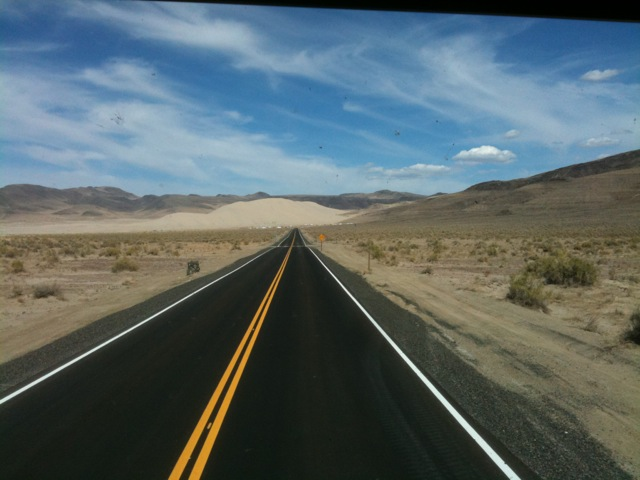
\includegraphics[scale=0.15]{images/paved_road.jpg}
        \end{figure}
      \end{itemize}
    \end{column}
    
    \begin{column}{0.5\textwidth}
      \begin{itemize}
      \item pollution
        \begin{figure}
	  \centering
	  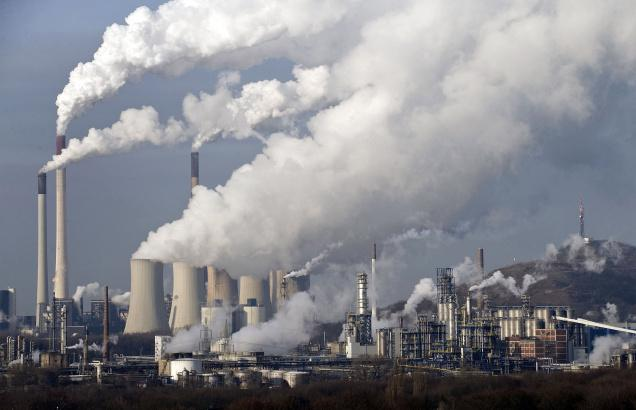
\includegraphics[scale=0.2]{images/pollution.jpg}
        \end{figure}
      \item Three metrics (in kt): \href{http://data.worldbank.org/indicator/EN.ATM.METH.KT.CE}{Methane}, \href{http://data.worldbank.org/indicator/EN.ATM.NOXE.KT.CE}{nitrous}, \href{http://data.worldbank.org/indicator/EN.ATM.CO2E.KT}{CO2}
      \end{itemize}
    \end{column}
  \end{columns}
\end{frame}


\begin{frame}{{\sc Climate Change} Model}{Checking conditions (equal variance \& normality)}
    \begin{figure}
      \centering
      \includegraphics[scale=0.05]{images/condition_plots/climate.jpeg}
      \caption{Left to right: \href{http://data.worldbank.org/indicator/EG.USE.ELEC.KH.PC}{\tt electricity.consumption}, \href{http://data.worldbank.org/indicator/EN.ATM.CO2E.KT}{\tt emissions.co2.kt}, \href{http://data.worldbank.org/indicator/EN.ATM.METH.KT.CE}{\tt emissions.methane}, \href{http://data.worldbank.org/indicator/EN.ATM.NOXE.KT.CE}{\tt emissions.nitrous}, \href{http://data.worldbank.org/indicator/IS.ROD.PAVE.ZS}{\tt paved.roads}}
    \end{figure}
\end{frame}

\begin{frame}{{\sc Climate Change} Model}{Log transform to fix unequal variance}
  \begin{itemize}
  \item all predictors improved drastically except {\tt paved.roads}
    \begin{figure}
      \centering
      \includegraphics[scale=0.06]{images/condition_plots/log_climate.jpeg}
      \caption{Left to right: \href{http://data.worldbank.org/indicator/EG.USE.ELEC.KH.PC}{\tt electricity.consumption}, \href{http://data.worldbank.org/indicator/EN.ATM.CO2E.KT}{\tt emissions.co2.kt}, \href{http://data.worldbank.org/indicator/EN.ATM.METH.KT.CE}{\tt emissions.methane}, \href{http://data.worldbank.org/indicator/EN.ATM.NOXE.KT.CE}{\tt emissions.nitrous}, \href{http://data.worldbank.org/indicator/IS.ROD.PAVE.ZS}{\tt paved.roads}}
    \end{figure}
  \end{itemize}
\end{frame}

\begin{frame}[fragile]{{\sc Climate Change} Regression}
\small
\begin{verbatim}
Coefficients:
                         Estimate Std. Error t value Pr(>|t|)    
(Intercept)             7.3364423  0.3095828  23.698  < 2e-16 ***
paved.roads             0.0192727  0.0042678   4.516 3.29e-05 ***
electricity.consumption 0.0001035  0.0000191   5.418 1.32e-06 ***
\end{verbatim}
\begin{itemize}
\item A one unit increase in \% of roads that are paved yields a 1.9\% increase in GDP per capita
\item BAD NEWS, $df = 56$, 155 observations deleted
\item Adjusted R-squared:  0.4841
\item With just {\tt electricity.consumption}, $df = 131$, $R^2 = 0.4362$, \& significant
\end{itemize}
\end{frame}

\begin{frame}[fragile]{{\sc Climate Change} Regression}{What about pollution?}
\small
\begin{verbatim}
Coefficients:
                     Estimate Std. Error t value Pr(>|t|)    
(Intercept)           6.14571    0.39413  15.593  < 2e-16 ***
log.emissions.co2.kt  0.25545    0.04114   6.209 3.37e-09 ***

Residual standard error: 1.449 on 187 degrees of freedom
  (25 observations deleted due to missingness)
Multiple R-squared:  0.1709,Adjusted R-squared:  0.1665 
\end{verbatim}
\begin{itemize}
\item CO2 was the only significant metric of pollution
\item $df = 187$!
\item A 1\% increase in CO2 emissions yields a 0.25\% increase in GDP per capita.
\end{itemize}
\end{frame}




% % % % % % % % % % % % % % % % % % % %
% % % % % % % % % % % % % % % % % % % %
% % % % % % % % % % % % % % % % % % % %
% SOCIAL DEVELOPMENT PREDICTOR
% % % % % % % % % % % % % % % % % % % %
% % % % % % % % % % % % % % % % % % % %
% % % % % % % % % % % % % % % % % % % %
\section{Social Development Model}

\begin{frame}{{\sc Social Development} Model}{\tt log(GDP.per.capita) $\sim$ \href{http://data.worldbank.org/indicator/SP.DYN.LE00.IN}{life.expect} + \href{http://data.worldbank.org/indicator/SL.TLF.0714.ZS}{child.labor} + \href{http://data.worldbank.org/indicator/SE.ADT.LITR.ZS}{literacy} + \href{http://data.worldbank.org/indicator/SM.POP.REFG.OR}{refugees}}
  \begin{columns}
    \begin{column}{0.5\textwidth}
      \begin{itemize}
      \item life expectancy
      \item child labor
        \begin{figure}
	  \centering
	  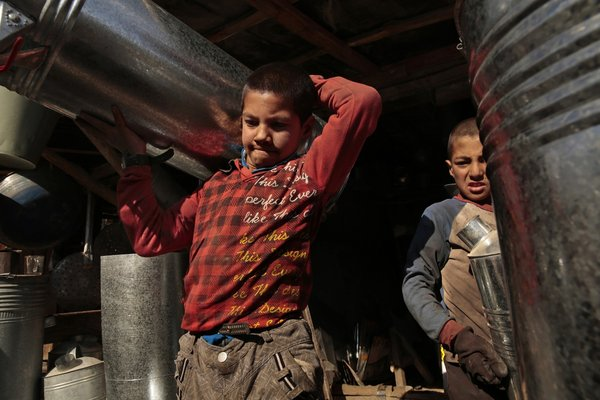
\includegraphics[scale=0.55]{images/child_labor.jpeg}
	  \caption{Child labor in metal shop, Kabul. LATimes.}
        \end{figure}
      \end{itemize}
    \end{column}
    
    \begin{column}{0.5\textwidth}
      \begin{itemize}
      \item literacy rates
      \item refugee population
        \begin{figure}
	  \centering
	  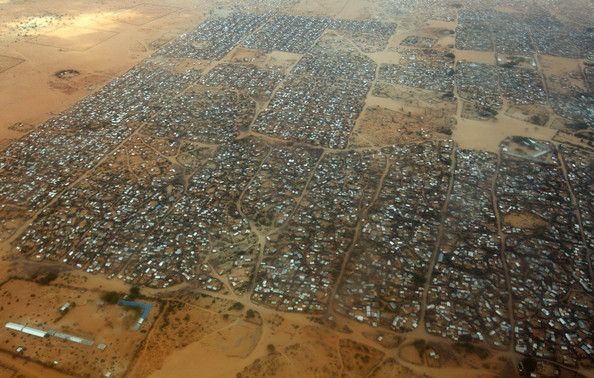
\includegraphics[scale=0.2]{images/refugee_camp.jpg}
	  \caption{Aerial view of refugee camp in Dadaab, Kenya.}
        \end{figure}
      \end{itemize}
    \end{column}
  \end{columns}
\end{frame}


\begin{frame}{{\sc Social Development} Model}{Checking conditions (equal variance \& normality)}
    \begin{figure}
      \centering
      \includegraphics[scale=0.08]{images/condition_plots/social_development.jpeg}
      \caption{Left to right: \href{http://data.worldbank.org/indicator/SL.TLF.0714.ZS}{\tt child.labor}, \href{http://data.worldbank.org/indicator/SP.DYN.LE00.IN}{\tt life.expect}, \href{http://data.worldbank.org/indicator/SM.POP.REFG.OR}{\tt refugees}, \href{http://data.worldbank.org/indicator/SE.ADT.LITR.ZS}{\tt literacy}}
    \end{figure}
\end{frame}

\begin{frame}{{\sc Social Development} Model}{Log transform to fix unequal variance}
  \begin{itemize}
  \item {\tt refugees} was the only improvable predictor
    \begin{figure}
      \centering
      \includegraphics[scale=0.25]{images/condition_plots/log_refugee.png}
      \caption{Left to right: \href{http://data.worldbank.org/indicator/SM.POP.REFG.OR}{\tt refugees}, \href{http://data.worldbank.org/indicator/SM.POP.REFG.OR}{\tt log.refugees}}
    \end{figure}
  \end{itemize}
\end{frame}

\begin{frame}[fragile]{{\sc Social Development} Regression}
\small
\begin{itemize}
\item {\tt child.labor} and {\tt literacy} had too few observations
\item $df = 177$!
\item A 1\% increase in life expectancy yields a 7\% increase in GDP per capita.
\end{itemize}
\begin{verbatim}
Coefficients:
                 Estimate Std. Error t value Pr(>|t|)    
(Intercept)     -19.88804    2.30273  -8.637 3.31e-15 ***
log.life.expect   6.98123    0.53375  13.080  < 2e-16 ***
log.refugees     -0.13567    0.02321  -5.846 2.37e-08 ***
---
Signif. codes:  0 ‘***’ 0.001 ‘**’ 0.01 ‘*’ 0.05 ‘.’ 0.1 ‘ ’ 1

Residual standard error: 0.9681 on 177 degrees of freedom
  (34 observations deleted due to missingness)
Multiple R-squared:  0.6326,Adjusted R-squared:  0.6284 
F-statistic: 152.4 on 2 and 177 DF,  p-value: < 2.2e-16
\end{verbatim}

\end{frame}



% % % % % % % % % % % % % % % % % % % %
% % % % % % % % % % % % % % % % % % % %
% % % % % % % % % % % % % % % % % % % %
% SCIENCE PREDICTOR
% % % % % % % % % % % % % % % % % % % %
% % % % % % % % % % % % % % % % % % % %
% % % % % % % % % % % % % % % % % % % %
\section{Science Model}

\begin{frame}{{\sc Science} Model}{\tt log(GDP.per.capita) $\sim$ \href{http://data.worldbank.org/indicator/TX.VAL.TECH.MF.ZS}{high.tech} + \href{http://data.worldbank.org/indicator/GB.XPD.RSDV.GD.ZS}{r.n.d} + \href{http://data.worldbank.org/indicator/IP.JRN.ARTC.SC}{journals}}
  \begin{itemize}
  \item high tech exports (\% of manufactured exports)
  \item science journals
  \item research and development (\% of GDP)
    \begin{figure}
      \centering
      \includegraphics[scale=0.5]{images/country_maps/science/map_science.jpeg}
    \end{figure}
    
  \end{itemize}
\end{frame}


\begin{frame}{{\sc Science} Model}{Checking conditions (equal variance \& normality)}
    \begin{figure}
      \centering
      \includegraphics[scale=0.1]{images/condition_plots/science.jpeg}
      \caption{Left to right: \href{http://data.worldbank.org/indicator/TX.VAL.TECH.MF.ZS}{\tt high.tech}, \href{http://data.worldbank.org/indicator/GB.XPD.RSDV.GD.ZS}{\tt r.n.d}, \href{http://data.worldbank.org/indicator/IP.JRN.ARTC.SC}{\tt journals}}
    \end{figure}
\end{frame}

\begin{frame}{{\sc Science} Model}{Log transform to fix unequal variance}
    \begin{figure}
      \centering
      \includegraphics[scale=0.3]{images/condition_plots/log_science.png}
      \caption{Left to right: \href{http://data.worldbank.org/indicator/TX.VAL.TECH.MF.ZS}{\tt log.high.tech}, \href{http://data.worldbank.org/indicator/GB.XPD.RSDV.GD.ZS}{\tt log.research}, \href{http://data.worldbank.org/indicator/IP.JRN.ARTC.SC}{\tt log.journals}}
    \end{figure}
\end{frame}


\begin{frame}[fragile]{{\sc Social Development} Regression}
\small
\begin{itemize}
\item Significant interaction terms involving \emph{high tech exports}!
\item $df = 72$, not bad\dots
\item a 1\% increase in high tech exports yields a 2.11\% increase in GDP per capita
\end{itemize}
\begin{verbatim}
Coefficients:
                           Estimate Std. Error t value Pr(>|t|)    
(Intercept)                 3.78461    1.05710   3.580 0.000620 ***
log.high.tech               2.11464    0.42922   4.927 5.16e-06 ***
log.research               -0.75793    0.33857  -2.239 0.028270 *  
log.journals                0.66064    0.15078   4.382 3.93e-05 ***
log.high.tech:log.research  0.54359    0.09804   5.545 4.59e-07 ***
log.high.tech:log.journals -0.23703    0.06301  -3.762 0.000341 ***
log.research:log.journals   0.02121    0.04545   0.467 0.642206    
---
Signif. codes:  0 ‘***’ 0.001 ‘**’ 0.01 ‘*’ 0.05 ‘.’ 0.1 ‘ ’ 1

Residual standard error: 0.8903 on 72 degrees of freedom
  (135 observations deleted due to missingness)
Multiple R-squared:  0.6545,Adjusted R-squared:  0.6258
\end{verbatim}
\end{frame}






% % % % % % % % % % % % % % % % % % % %
% % % % % % % % % % % % % % % % % % % %
% % % % % % % % % % % % % % % % % % % %
\section{Conclusion}
\begin{frame}{Conclusion}
\begin{itemize}
\item No full model.
  \begin{itemize}
    \item Could not combine all predictors.
    \item Too much multicollinearity.
  \end{itemize}
\item Instead, we have provided {\bf FIVE} robust models for {\bf explaining} why some countries are wealthier than others.
\end{itemize}
\end{frame}


% % % % % % % % % % % % % % % % % % % %
% % % % % % % % % % % % % % % % % % % %
% % % % % % % % % % % % % % % % % % % %
\section{Future Extensions}

\subsection{Stepwise Selection of Predictors}

\begin{frame}{Future Extension}{The {\tt step} function}
\begin{itemize}
\item Perform logistic and AOV regressions.
\item Use the {\tt step} function to automatically select predictors.
\item Caveat: {\tt step} yields an exceptional model with an $R^2$ value $> 99.9$\%.
$$\textrm{GDP per cap} = \beta_0 + \beta_1 \cdot \mathrm{imports} + \beta_2 \cdot \mathrm{exports} + \beta_3 \cdot \textrm{gov spending}$$
\end{itemize}
\end{frame}


\end{document}


